\Chapter{SYNTHETIC DATA GENERATION}\label{sec:Syn}



Generally to validate a proposed approach, simulated data is the best candidate because all the parameters could be predefined. Once the simulated data is generated with predefined parameters, the model can be trained over the generated data. This may be the strongest benefit of synthetic data in model fitting. 

The framework of this study relies on synthetic data. We rely on simulated data for all experiments at the first place. Although it lacks the external validity of real data, it remains the most reliable means of obtaining test results data for which the underlying, parameters such as latent skills structure is perfectly known. Every model studied here can be considered \textit{generative}, to the extent that they can generate synthetic data.  The data generation process of each model share common parameters which are: number of items, number of students, total success rate and data distribution but other parameters vary according to different techniques.  The generation process for each model is described below.


\section{POKS}
The method that generates synthetic dataset based on the POKS model requires a knowledge structure (KS). In this process the KS can be obtained from a real data set which allows us to make a better comparison of the results. It can also be generated as a random KS. The graphical demonstration of knowledge structure is a directed tree which shouldn't have any loop, therefore in the random generation of KS this issue should be considered otherwise it violates the definition of KS. There are other input parameters which can make the random generation more specific like the number of links and number of independent trees in a KS. Applying these parameters will change the item variance in the test result matrix. In order to avoid loops in knowledge structure graph, we create an upper triangular adjacency matrix with random links. Once the KS adjacency matrix is created , we can assign values to each item that contributes with the initial odds of each node and odds ratio between a pair of nodes.

%The second approach  is using probabilities for each node and a ratio for each pair for nodes which represent the strength of the link.  Based on the knowledge structure that has been picked we can also assess a set of initial probability for each node where a parent node gets a lower initial probability than its children. For inference in POKS framework to calculate the node's probability, we use standard Bayesian posteriors under the local independence assumption. The probability update for node $H$ given $E_1$,... $E_n$ can be written in following posterior odds form :

The approach for assigning values to each sample is using probabilities for each node and a ratio for each pair for nodes which represent the strength of the link.  Based on the knowledge structure that has been picked we can also assess a set of initial probability for each node where a parent node gets a lower initial probability than its children. Inference in the POKS framework to calculate the node's probability relies on standard Bayesian posteriors under the local independence assumption. The probability update for node $H$ given $E_1$,... $E_n$ can be written in following posterior odds form :
\begin{equation}
O(H|E_1,E_2, ... , E_n) = O(H) \prod_{i}^{n} \frac{P(E_i|H)}{P(E_i | \overline{H})}
\label{EQPOKSratio}
\end{equation}
where odds definition is $O(H|E) = \frac{P(H|E)}{1-P(H|E)}$. If evidence $E_i$ is negative for observation $i$, then the ratio $\frac{P(\overline{E_i}|H)}{P(\overline{E_i}|\overline{H})}$ is used.

All the parameters containing Partial Order structure, initial odds and odds ratio can also be obtained form a real dataset. For the case that these values are not predefined we need to assign random values with respect to the defined partial order structure. Once these values are defined, we can pick a node to sample with it's initial odds and consequently update it's neighbors' odds with equation~\ref{EQPOKSratio}. This process could be continued until there exists no node to sample.

The only way to control the total test result successrate and student/item score variance is to apply changes on the initial odds of nodes where we use for sampling student test result. For student scores variance, for each student the initial odds can be scaled such that the distribution of the initial odds stays the same for example we can double all the initial odds to represent a student with higher success rate. Changing the initial odds that follows a specific distribution will create a dataset in which the item variance is following that distribution. For overall successrate the initial odds can be scaled independent from students or item perspective, for example tripling all initial odds for all students will result in a higher success rate than the default values.

\section{IRT}

Equation~\ref{IRTEQ} shows the probability of a student given the ability of $\theta$ to success item $j$ which has the difficulty of $b_j$ and discrimination of $a_j$ based on IRT-2PL model. To generate a dataset that follows this model, we need to generate a sample of students with different abilities and items with different difficulties and discriminations. 
\begin{equation}
P(X_j\!=\!1\;|\;\theta) = \frac{1}{1+e^{-a_j(\theta-b_j)}}
\label{IRTEQ}
\end{equation}
\[-4 < \theta < 4\]
\[-3 < b_j < 3\]

Students ability to answer questions and item difficulty are generated by a normal distribution with the mean of $0$ and standard deviation of $1.25$ with respect to their boundaries. Discrimination (slope or correlation) representing how steeply the rate of success of individuals varies with their ability. In IRT-2PL, the values for discrimination are following a Poisson distribution with lambda parameter set to 10 that kept most values between 0.5 and 3 . Note however that for the purpose of synthetic data generation, we rely on the more general IRT-2PL model in order to make this data more realistic.

Item discrimination is a parameter that is learnt from training set. A perfect dataset that doesn't have any noise estimates this parameter with extremely large or small values(for example $300$ or $-300$)  which results in an unrealistic outcome prediction. For this purpose we add small amount of noise to prevent this condition.

\section{Linear NMF Conjunctive}

The very first step to generate simulated test result for linear models is to define a Q-matrix that maps $k$ skills to $n$ items. The Q-matrix can be an expert predefined matrix or a random generated matrix. In the case of unavailable predefined Q-matrix, we defined a Q-matrix that provides all the possible combination of $k$ skills with a maximum of $Max$ skills per item, and at least one skill per item. A total of $\sum\limits_{k=1}^{Max} \dbinom{n}{k}$ items span this space of combinations for example $21$ items for 6 skills and maximum 2 skills per item. This matrix is shown in Figure~\ref{figqmatrixandResutM}. Items 1 to 15 are two-skills and items 16 to 21 are single-skill. Once the Q-matrix is created we can randomly replicate or eliminate some items to adjust the number of items to the desired number. 

\begin{figure}[ht]
\centering

\subfigure[Q-matrix of 6 skills]{
   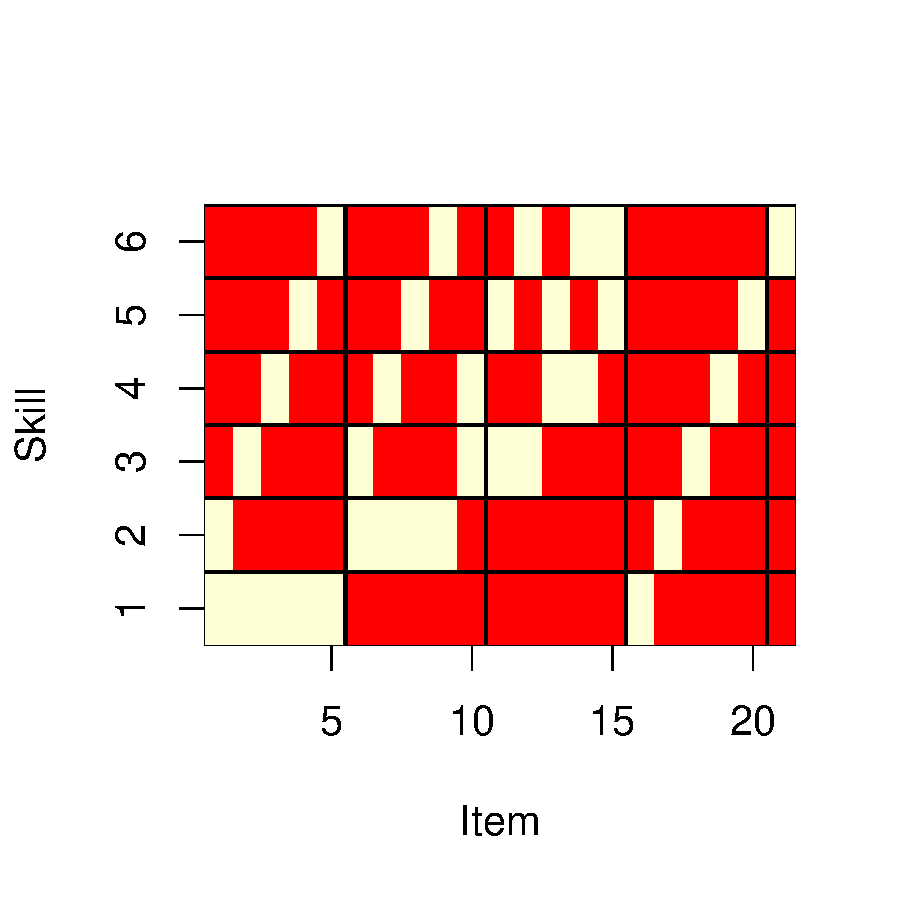
\includegraphics[scale =0.5] {ExpectedQ.pdf}\label{PerfectQ}
 }\quad
 \subfigure[Synthetic data of 100 students with 10\% slip and 20\% guess factor]{
   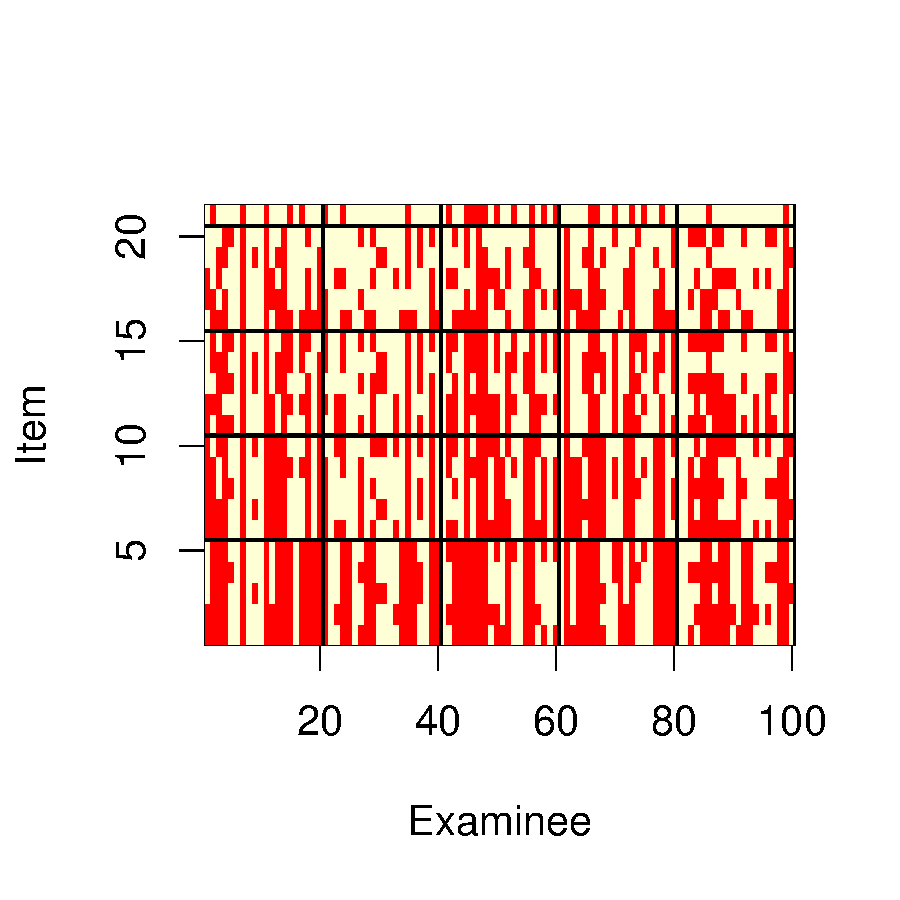
\includegraphics[scale =0.5] {ResultM.pdf}
 }
\caption{Q-matrix and an example of simulated data with this matrix.  pale cells represent 1's and red ones represent 0's.}
\label{figqmatrixandResutM}
\end{figure}

There are two ways to apply item variance in the simulated data and both of them are based on manipulating the values of the Q-matrix. Applying skills difficulty on skills would transfer the difficulty to items that have this skill. The other method is to consider the same weight for skills difficulty but controlling the item variance by assigning different number of skills to items. For example items with 1 skill would become easier to answer comparing to items with two or more skills where skills difficulty is the same for all skills. 

The second step is to create a student skills mastery matrix which maps $k$ skills to $m$ students. In terms of ability for examinees we assigned random values to skills for students but  student variance show up as the variance in number of skills across examinees. At the same time we can apply the overall success rate on the skill mastery matrix using a threshold to discrete the assigned values in skills mastery. 

Once the Q-matrix and Skills mastery matrix is created we can produce the test result matrix with equation~(\ref{eq:6}). The last step is to add slip and guess factors which are set as constant values across items.

A sample of the results matrix is given in figure~\ref{figqmatrixandResutM} where pale cells represent a value of 1 and red cells are 0. Examinee ability shows up as vertical patterns, whereas skills difficulty creates horizontal patterns. As expected, the mean success rate of the 2-skills items 1 to 15 is lower than the single skill items 16 to 21.

\section{Linear NMF Additive}

The process to create synthetic data based on additive type of Q-matrix is almost the same as Conjunctive one. The difference is on the interpretation of the Q-matrix that changes the step where the result matrix is producing.

For this case each cell in the Q-matrix should be normalized on the bases of items. Although each skill has a specific weight to success an item but in our experiment we consider equal weight for all skills of an item. For this purpose all the values assigning to each item in Q-matrix should be divided by the number of involved skills for that item.

\begin{figure}[h]
\begin{tabular}{c}
\subfigure[{Additive Q-matrix\label{figNMFAddQM}}]{\begin{footnotesize}
$\begin{array}{ccc}
 && \textrm{items}\\

\mathrm{\begin{sideways}skills\end{sideways}} & & \left[\begin{array}{cccccccccccccccccc}

0.5&0.00&0.25&0.33&0.33&0.33&0.00&0.5&0.5&0.5&0.0&0.0&0.0&1&0&0&0\\
0.0&0.33&0.25&0.33&0.33&0.00&0.33&0.5&0.0&0.0&0.5&0.5&0.0&0&1&0&0\\
0.0&0.33&0.25&0.33&0.00&0.33&0.33&0.0&0.5&0.0&0.5&0.0&0.5&0&0&1&0\\
0.5&0.33&0.25&0.00&0.33&0.33&0.33&0.0&0.0&0.5&0.0&0.5&0.5&0&0&0&1


\end{array}\right]
\end{array}$
\end{footnotesize}
}\\
\begin{tabular}{cc}
\subfigure[Raw Result matrix ]{
   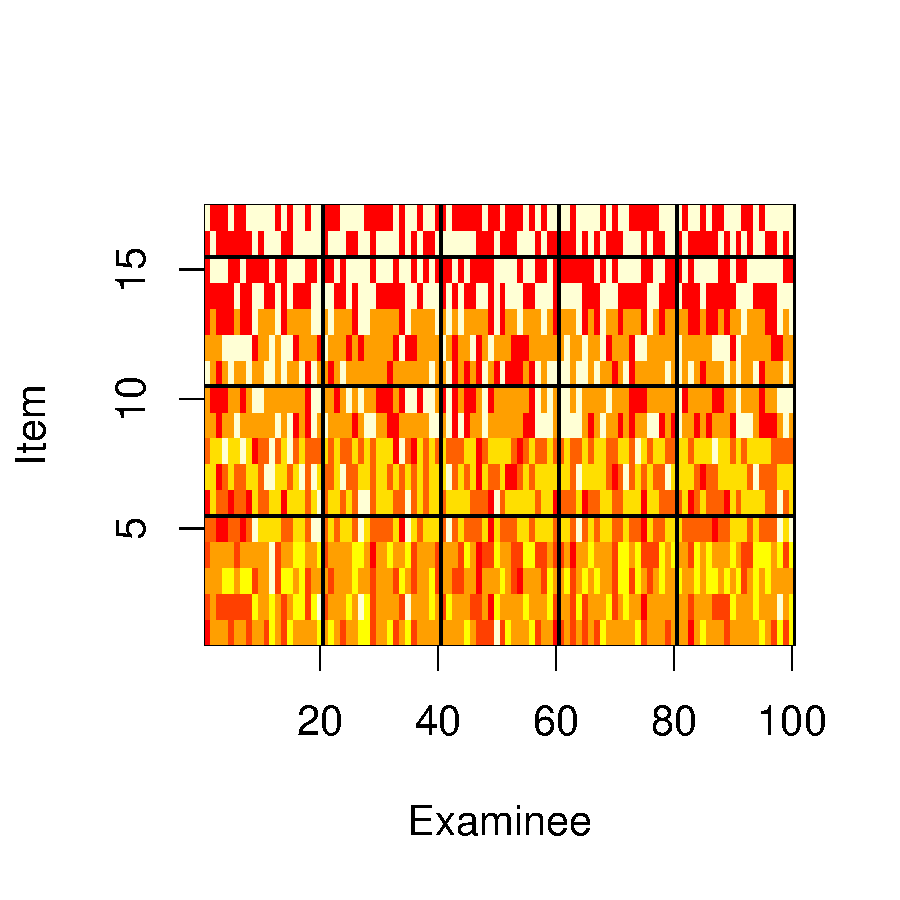
\includegraphics[scale =0.5] {NMFAddNonNoisy.pdf}\label{NMFAddNonNoisy}
 }\quad
&
\subfigure[Discretized result matrix with 20\% slip and 10\% guess factor]{
   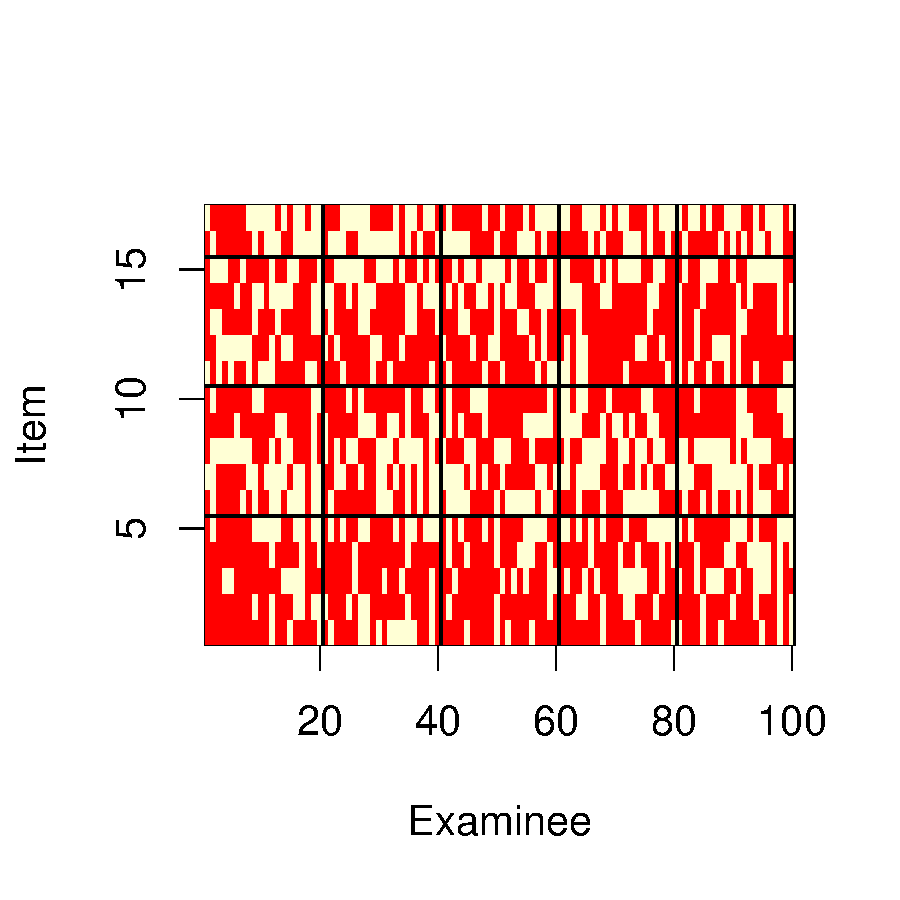
\includegraphics[scale =0.5] {NMFAddNoisy}\label{NMFAddNoisy}
 }\quad
\end{tabular}
\end{tabular}
\caption{Additive model of Q-matrix and Corresponding synthetic data}
\label{figNMFAddgen}
\end{figure}

Figure~\ref{figNMFAddQM} shows an additive type of Q-matrix and figure~\ref{NMFAddNoisy} is the result of cross product of this matrix to a students skills mastery matrix. Since the model is additive, there are some pale cells and the paler a cell is, the more chance a student has to success the question. In conjunctive model the result matrix is either $0$ or $1$. 

\section{DINA/DINO}
These models are also categorized as linear models that use a Q-matrix. The Q-matrix can be predefined for a better comparison or can be synthetic. For synthetic Q-matrix we use the same method as described before. At the same time we can control the number of skills and items in generation of a Q-matrix.

Equation~\ref{DinoEQ3} requires three parameters to predict a test outcome. In our experiment we create a sequence of values for guess and slip in the range of $0$ and $0.2\%$. Examinee's skills can be generated by a normal distribution which should match the number of skills presented in the Q-matrix. The difference between creation of skills mastery matrix in DINA/DINO and NMF is the way that skills are appearing for each student. In DINA/DINO there is a predefined set of possible combination of skills that can be used in skills mastery for each student. For example for 3 skills, this set can have maximum 8 combination. There is a distribution that is assigned to this set which defines the probability of appearance for each combination in the skills mastery matrix. 
\begin{equation}
 P(X_{ij} \!=\! 1 \; | \; \xi_{ij}) \,=\, (1-s_j)^{\xi_{ij}} g_j^{1-\xi_{ij}}
\label{DinoEQ3}
\end{equation}
We can apply total success rate during the creation of student's skills mastery matrix where students skills define the success rate of a dataset. Since these models are behaving based on a single value that represents student ability, we need to calculate an array of abilities for each item given a set of skills for an student. In DINO we use a disjunction between skills of an item and skills of a student to determine whether the student has the ability or not where for DINA a conjunction applies.

